\chapter{Activity Classification in Videos}
One of the main objectives of this research is to provide a reliable method for
activity classification in videos. For this thesis, two activities of interest
to the College of Education are studied: when students are writing and when they
typing. The idea being that if we can prove that classification using ViDA works
for simple activities, we can extend the system to handle other activities just
by changing the training data and training a new classifier on that data, making
the system extremely flexible. This chapter reviews the basic techniques that
are used for reducing the feature space of videos so that any machine learning
algorithm, such as an SVM, can be used to classify the activities. It explains
the basic implementation of the Farneback optical flow algorithm
\cite{farneback2003two}, also known as dense optical flow, how the optical flow
features are further reduced, and finally the methods used to classify the
activity in the video.

\section{\label{section:optical_flow_methods}Optical Flow Methods}
In this thesis we attempt to classify two types of activities in video,  typing
and writing. Since both of these activities involve motion, i.e. a change of
apparent structure position from one video frame to the next, optical flow
algorithms  are a suitable tool for attempting to extract germane features from
the video.

Currently, there are several varieties of optical flow algorithms that have been
published. We use both Lucas-Kanade \cite{lucas1981iterative} and the Farneback
\cite{farneback2003two}  optical flow algorithms to attempt to extract
important motion features from the AOLME videos. Although as we see with our
experiments, that the Farneback algorithm is better suited for pulling out
motion features that our unique to the particular motion for which we attempt
to find in our videos. In either case, both algorithms attempt to solve
Equation \ref{eq:delta_image}

\begin{equation}
I(x,y,t) = I(x+dx, y+dy, t+dt)
\label{eq:delta_image}
\end{equation}

where $I$ is the the image, $x$ \& $y$ are the column row coordinates
respectively, and $t$ is the time between two adjacent image frames. Taking the
Talylor series expansion of Equation \ref{eq:delta_image} results in Equation
\ref{eq:taylor_expansion}


\begin{equation}
f_x u + f_y v + f_t = 0
\label{eq:taylor_expansion}
\end{equation}

where

\begin{equation}
f_x = \frac{\partial f}{\partial x} \; ; \; f_y = \frac{\partial f}{\partial y} \\
u = \frac{dx}{dt} \; ; \; v = \frac{dy}{dt}
\label{eq:taylor_expansion_partial}
\end{equation}

 Equation is \ref{eq:taylor_expansion_partial} is known as the Optical Flow
 equation. The object is determine what $u$ and $v$ are given that $f_x$ and
 $f_y$ are the image gradients and $f_t$ is the time gradient. Since in Equation
 \ref{eq:taylor_expansion} we have two unknowns, we cannot solve the system
 without additional constraints. This is known as the \textit{aperture problem}.
 Both the Lucas-Kanade method and the Farneback method attempt to estimate this
 problem. Lucas-Kande attempts to reframe the problem such that we have an
 overdetermined system, solving it and then providing motion vectors for only
 features that move. The Farneback solution, on the other hand, argues that is
 possible to solve the \textit{aperture problem} by first approximating each
 neighborhood of both frames with quadratic polynomials, and then estimating the
 displacement fields between the frames using polynomial expansion. Rather than
 providing only a few motion vectors, the Farneback method provides dense
 optical flow. That is to say that there is a motion vector for every pixel
 between the frames \cite{farneback2003two}.

\subsection{\label{subsection:lucas_kanade} Lucas-Kanade Method} For this
thesis, we leverage a common C++ library that has already implemented a
specialized version of the general Lucas-Kanade algorithm which uses pyramids to
solve the optical flow at different scales of motion
\cite{bouguet2001pyramidal}. This algorithm is provided freely in a C++ computer
vision library known as OpenCV \cite{itseez2015opencv}. Essentially, this
algorithm is much like the original paper published by Lucas and Kanade, but it
solves the issue of large motions between frames. By definition, the Lucas-Kande
method assumes that the displacement of features in the image between two frames
is small and roughly constant within a pixel neighborhood. This algorithm, then,
by definition cannot handle large motions between frames, and hence the algorithm
presented in \cite{bouguet2001pyramidal} attempts to more robustly solve
optical flow and is the algorithm that is implemented in the OpenCV \cite{itseez2015opencv}
library. In our software, we use two OpenCV library calls, \texttt{goodFeaturesToTrack}
and \texttt{calcOpticalFlowPyrLK}. The first function is used to find features
that can be easily tracked from one frame to the other using the Shi-Tomasi
algorithm \cite{shi1994good}. The next method then calculates the optical flow
between the good points using the pyramidal implementation of the Lucas-Kanade
algorithm \cite{bouguet2001pyramidal}. Algorithm \ref{alg:lk_flow} outlines the general
program flow for calculating motion vectors in ViDA.

\begin{algorithm}
\caption{Calculating Lucas-Optical Flow from Videos}
\label{alg:lk_flow}
\begin{algorithmic}[1]
\Procedure{CalculateVectors}{$frame1$, $frame2$}
  \If{\text{$track\_points\_initialized$}}
  	\State $opticalflow \gets \texttt{calcOpticalFlowPyrLK}(track\_points, frame1, frame2)$
  \Else
  	\State $track\_points \gets \texttt{goodFeaturesToTrack}(frame1)$
	\State $track\_points\_initialized \gets True$
	\State $optical\_flow \gets  \texttt{CalculateVectors}(frame1, frame2)$
  \EndIf
  \Return $optical\_flow$
\EndProcedure
\end{algorithmic}
\end{algorithm}

\subsection{\label{subsection:farneback_method} Farneback Method}
Again, we leverage the C++ OpenCV library to calculate the motion vectors for
Farneback optical flow. Unlike the previous method, the Farneback algorithm does not require
any track points to estimate motion vectors because it is a dense optical flow
algorithm, i.e. 100\% of the pixels has an associated optical flow vector. The
main idea behind calculating the motion vectors in this method, is to use
polynomial expansion for a neighborhood of pixels \cite{farneback2003two} and
then use that estimation to find a global translation between the two frames. This
essentially aids with global background movement. The main algorithm used in ViDA
is similar to Algorithm \ref{alg:lk_flow} but contains fewer steps since there
is no need to get good features to track. The Farneback implementation is shown
in Algorithm \ref{alg:farneback}.

\begin{algorithm}
\caption{Calculating Farneback Flow from Videos}
\label{alg:farneback}
\begin{algorithmic}[1]
\Procedure{CalculateVectors}{$frame1$, $frame2$}
  \State $optical\_flow \gets \texttt{calcOpticalFlowFarneback}(frame1, frame2)$\\
  \Return $optical\_flow$
\EndProcedure
\end{algorithmic}
\end{algorithm}

\subsection{\label{subsection:comparison}Comparison of Methods}
We implemented the Lucas-Kanade method first in our research because in general,
performance is a concern and, as long as not too many features or
too few features are detected, the Lucas-Kanade algorithm will be faster
\cite{de2015choosing}. Despite this fact, we found that our classifier did
not perform as well on features extracted from the Lucas-Kanade method, as it
did using the Farneback method. As a result, most of the results in this thesis
have been calculated with Farneback optical flow unless otherwise specified.

\section{\label{section:feature_extraction}Feature Extraction from Optical Flow}
The \texttt{CalculateVectors} function in both Algorithm \ref{alg:lk_flow} and
\ref{alg:farneback} returns several dense matrices that represent the features
that we can extract from the optical flow output. These features are magnitude,
orientation, x direction and y direction of the optical flow features. These
are ultimately the features that we use to train and classify using an SVM. However,
if we had two $N \times M$ video frames as the input, we now have $4 \times N \times M$
features. Clearly we have not yet reduced the input feature space. Thus, based
on information that we know \textit{a-priori}, we can reduce our feature space
significantly.

In the case of typing and writing, we know we can expect there to be motion from
one frame to the next. We don't know by how much, but we do know that it is not
zero. Using this knowledge, we can then threshold the optical flow vectors that
we get back from Algorithms \ref{alg:lk_flow} and \ref{alg:farneback}. The
threshold value used was empirically calculated from doing multiple runs on the
AOLME videos. We found we got the best results by only retrieving
optical flow vectors with a magnitude greater than 75\% of the max value. The set
of Equations in \ref{eq:optical_threshold} illustrate this idea.

\begin{align}
  \label{eq:optical_threshold}
  \begin{split}
  \mathbf{V} &= (\mathbf{V_x}, \mathbf{V_y}) \\
  \mathbf{V_m} &=
  \begin{cases}
    1, & \text{if } \|\mathbf{V}\| \geq \max( \|\mathbf{V}\|) \times 0.25 \\
    0, & \text{otherwise}
  \end{cases}
  \end{split}
\end{align}

where $\mathbf{V_x}$ and $\mathbf{V_y}$ are the optical flow vectors in the
x and y directions respectively. $\mathbf{V_m}$ is the bit mask that is
then used to extract the subset of data from each of the dense matrices.

\begin{align}
  \label{eq:subset}
  \begin{split}
  \text{Let: } \\
  \|\mathbf{V\prime}\| &= \|\mathbf{V}\| \circ \mathbf{V_m}\\
  \mathbf{V_x\prime} &= \mathbf{V_x} \circ \mathbf{V_m}\\
  \mathbf{V_y\prime} &= \mathbf{V_y} \circ \mathbf{V_m}\\
  \mathbf{\Phi\prime} &= \mathbf{\Phi} \circ \mathbf{V_m}
\end{split}
\end{align}

Using the optical flow bitmask, $\mathbf{V_m}$, we can then extract features
from each one of our dense matrices using the Hadamard product as shown in
Equation \ref{eq:subset}, where $\|\mathbf{V\prime}\|,
\mathbf{V_x\prime},\mathbf{V_y\prime}, \mathbf{\Phi\prime}$ are subset matrices
for the magnitude, x and y direction and orientation respectively. We have now
reduced the feature space somewhat, but depending the size of the video and the
amount of entropy per frame pair, we could still have a significant amount of
data to process for classification.

In addition to extracting generic vectors from the video, we also add
geometrical centroids, blob orientation and background motion around the blobs
to the optical flow statistics being used for classification. We implement these
methods to attempt to leverage information that could be useful during
classification. In order to calculate the geometrical centroids and orientations
of each blob, we use some well known algorithms available in OpenCV,
\texttt{connectedComponentsWithStats} and \texttt{findContours}
\cite{itseez2015opencv}. \texttt{connectedComponentsWithStats} is a function
that allows us to compute the centroid for each blob of connected pixels. The
input to this function is our binary mask image, $\mathbf{V_m}$. Once we have
all the connected blobs, we can then calculate the orientation of each one of
those blobs using \texttt{findContours} in combination with with
\texttt{fitEllipse}. The full implementation of this algorithm is outlined in
Appendix \ref{ap:centroids}. The final step is to then dilate each blob, and
then calculate the optical flow statistics in the difference region. Appendix
\ref{ap:dilate}. Figure \ref{fig:orient_cent} illustrates the idea of acquiring
the centroid and orientation of the blobs from $\mathbf{V_m}$.

\begin{figure}[h]
  \label{fig:orient_cent}
  \centering
  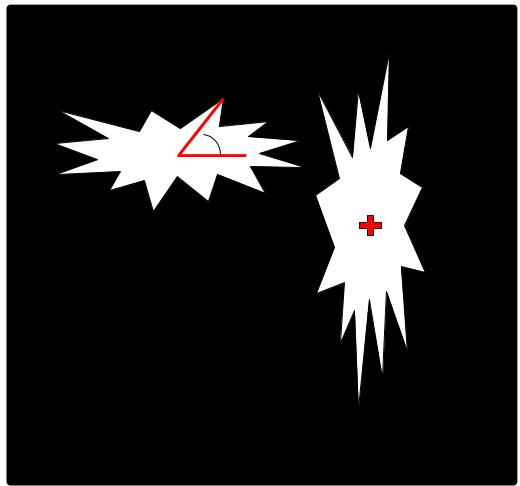
\includegraphics[width=8cm]{figures/cent_and_orient}
  \caption{Example of orientation measurement on the left, and the centroid calculation on the right.}
\end{figure}

When the previous optical flow features have been generated, their values are then
organized into a probability density function (PDF) with 25 bins. That is to say that
each frame pair generates a PDF and that PDF is accumulated for every subsequent
frame in the video sequence. When our software reaches the end of the video file,
a normalized, cumulative distribution function (CDF) is calculated and output
for each vector. So for each input video there will be one CDF with 25 bins
for blob orientation, blob centroid x and y, motion vector magnitude, motion
vector orientation and background motion vector magnitude. Figure \ref{fig:extract_flow}
clearly illustrates this concept.

\begin{figure}[h]
  \label{fig:extract_flow}
  \centering
  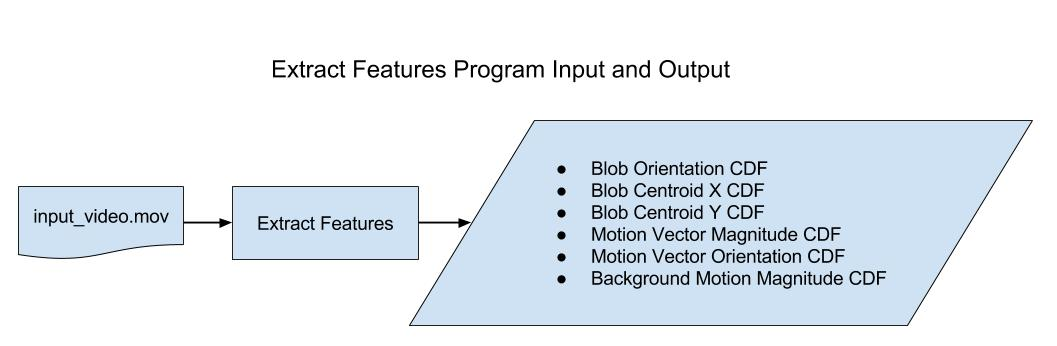
\includegraphics[width=14cm]{figures/extract_features_flow}
  \caption{Flow of the extract features program. For every input video, it will
  return a CDF with 25 bins for each of the extracted features from the motion
  vectors}
\end{figure}

\section{\label{section:the_data}The AOLME Dataset}
The AOLME dataset is an enormous repository of over 900 hours of video
recordings of students [reference needed]. The videos contain students
interacting with facilitators, their peers and computers to write code in
Python on the Raspberry Pi.  The dataset is wealth of information but difficult
to exploit in its current state.  The data used for this thesis is a subset of
the entire AOLME dataset. By hand, we have selected several videos and extracted
typing and writing clips from the original dataset and are using these as ground
truth for measuring the accuracy of our classification. Figure \ref{fig:typing_writing}
is representative of the features that have been extracted by hand.

\begin{figure}[h]
  \label{fig:typing_writing}
  \centering
  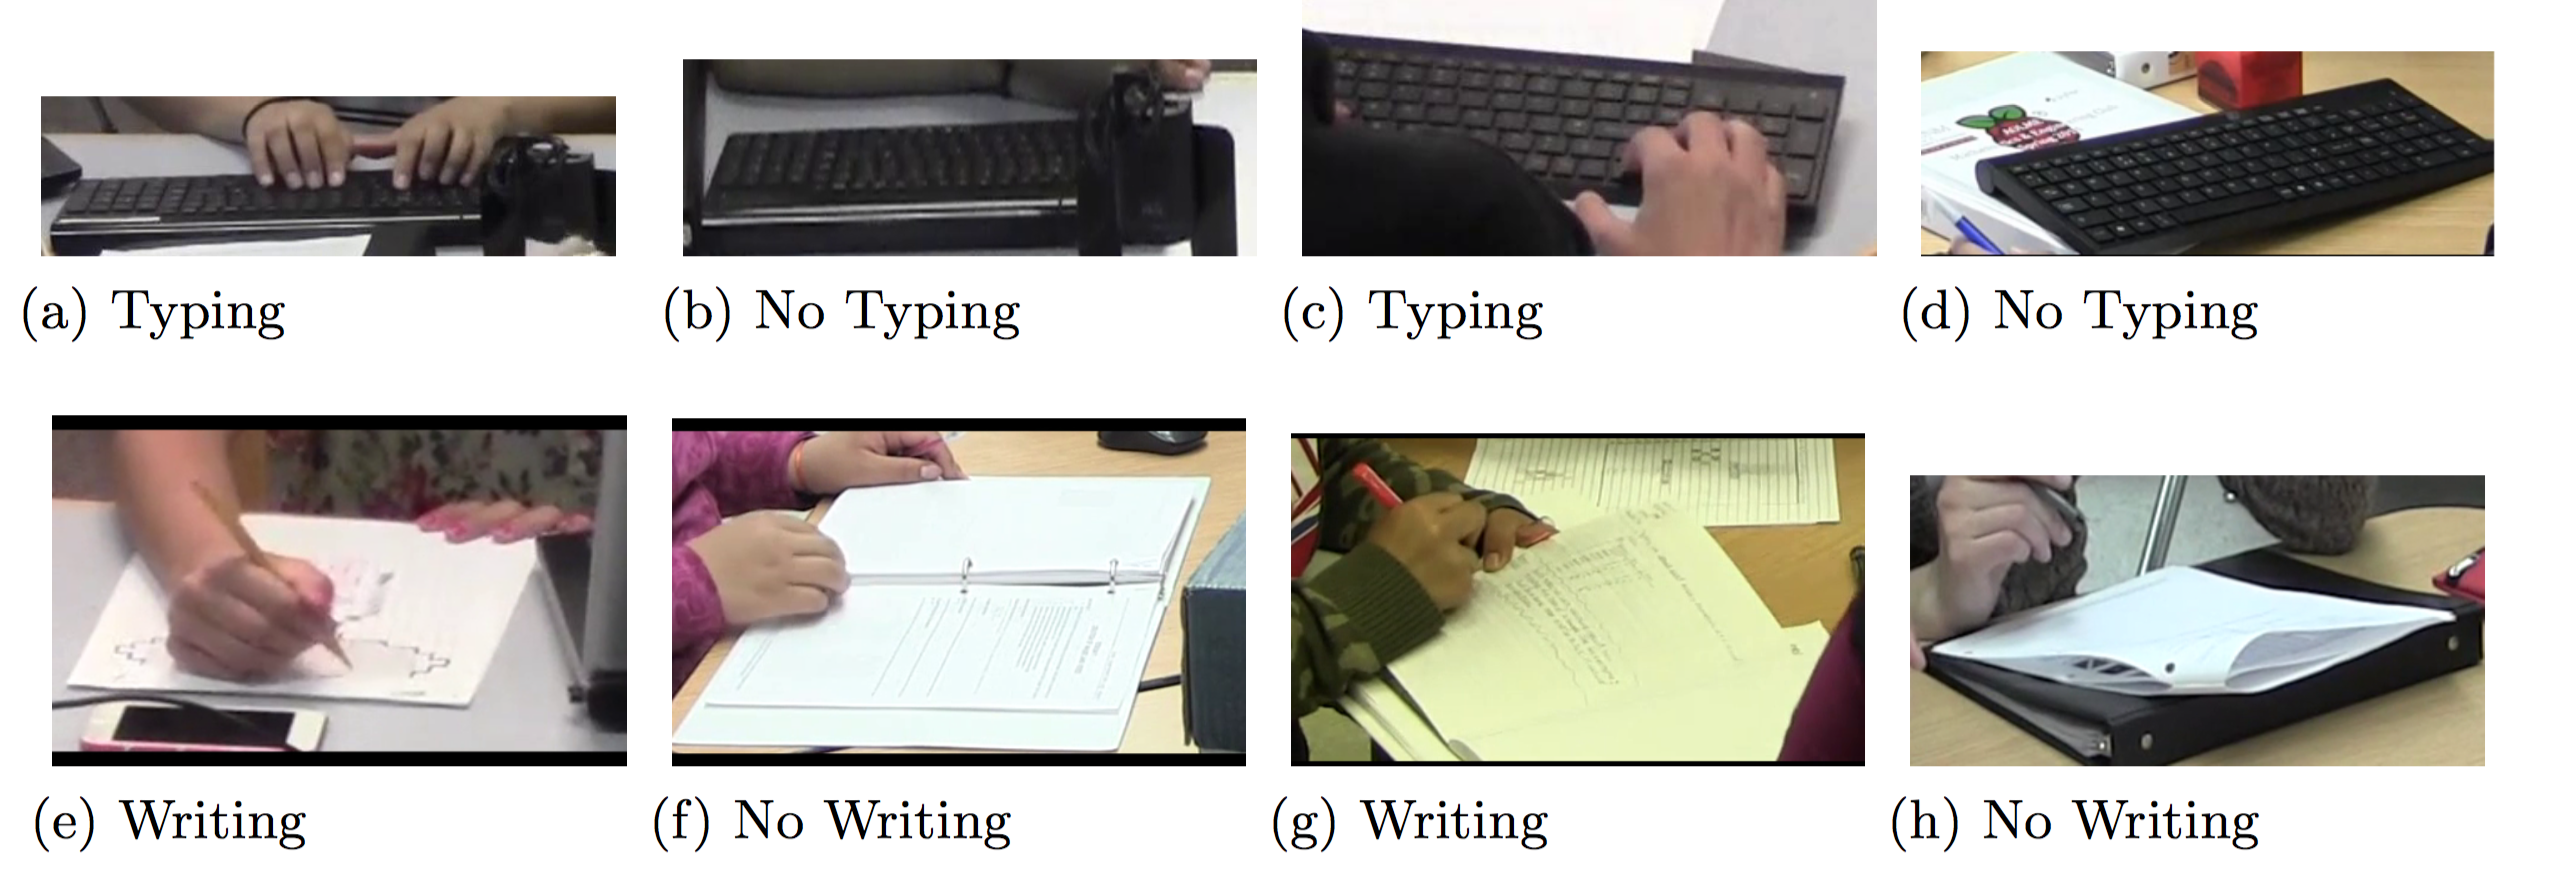
\includegraphics[width=\textwidth]{figures/typing_writing_clip}
  \caption{Example of features that have been manually extracted from the dataset
  for training and testing. For the above example, we need to classifiers for each
  activity to determine if the activity is being performed, or it is not.}
\end{figure}

As Figure \ref{fig:typing_writing} suggests, we are only using a cropped version
of the video. The reason is that we are not attempting to solve the tracking
problem in this thesis, only the classification problem. Hence, we assume that
the videos entering into our software have already been clipped and cropped with
the target activities inside of them and the corresponding lack of the activity.


\section{\label{section:classification}Classifying the Reduced Feature Space}
